\documentclass[aps,twocolumn]{revtex4-2}

\usepackage[english]{babel}

\usepackage{amsfonts,amsmath,bm,amssymb,revsymb,color,braket}
\usepackage{xcolor}
\usepackage{graphicx}
\usepackage[makeroom]{cancel}


\definecolor{bostonuniversityred}{rgb}{0.8, 0.0, 0.0}
\definecolor{dukeblue}{rgb}{0.0, 0.0, 0.61}
\definecolor{ao(english)}{rgb}{0.0, 0.5, 0.0}
\definecolor{darkmagenta}{rgb}{0.55, 0.0, 0.55}
\definecolor{armygreen}{rgb}{0.29, 0.33, 0.13}
\definecolor{coquelicot}{rgb}{1.0, 0.22, 0.0}
\definecolor{fucsiak}{rgb}{0.4, 0.08, 0.4}
\definecolor{airforceblue}{rgb}{0.36, 0.54, 0.66}
\definecolor{applegreen}{rgb}{0.55, 0.71, 0.0}
\definecolor{awesome}{rgb}{1.0, 0.13, 0.32}
\definecolor{burgundy}{rgb}{0.5, 0.0, 0.13}
\definecolor{cobalt}{rgb}{0.0, 0.28, 0.67}
\definecolor{aqua}{rgb}{0.0, 1.0, 1.0}
\definecolor{blue-green}{rgb}{0.0, 0.87, 0.87}

\usepackage[unicode=true,bookmarksnumbered,colorlinks=true, citecolor=burgundy, linkcolor=blue, urlcolor=cobalt]{hyperref}






\begin{document}

\title{Surface wave propagation against a steady ring current in a square basin}

\author{Maria D. Klimenko}

%\affiliation{Landau Institute for Theoretical Physics, Russian Academy of Sciences,\\1-A Akademika Semenova av., 142432 Chernogolovka, Russia}

\affiliation{Osipyan Institute of Solid State Physics, Russian Academy of Sciences,  \\ Chernogolovka, Moscow region, 142432 Russia}




\author{Ivan A. Vointsev}

\affiliation{National Research University Higher School of
	Economics, Faculty of Physics, Myasnitskaya 20, 101000
	Moscow, Russia}



\author{Sergey V. Filatov}

%\affiliation{Landau Institute for Theoretical Physics, Russian Academy of Sciences,\\1-A Akademika Semenova av., 142432 Chernogolovka, Russia}
\affiliation{Osipyan Institute of Solid State Physics, Russian Academy of Sciences,  \\ Chernogolovka, Moscow region, 142432 Russia}


\author{Sergey S. Vergeles}

\affiliation{Landau Institute for Theoretical Physics,
	Russian Academy of Sciences,\\1-A Akademika Semenova av.,
	142432 Chernogolovka, Russia}

\affiliation{National Research University Higher School of
	Economics, Faculty of Physics, Myasnitskaya 20, 101000
	Moscow, Russia}

\email{ssver@itp.ac.ru}



\begin{abstract}
% TODO: [Interpretation] Clarify how experimental eigenfrequencies were determined:
% the reported peaks are forcing harmonics, not independently measured resonances.
% Quantify the claimed frequency/profile agreement and identify the modes covered.
	Surface waves propagating against a ring current are observed experimentally and investigated theoretically. The ring current is generated in a square basin by a rotating disk mounted flush with the bottom. The same disk excites wave motion because its normal is slightly tilted relative to the vertical axis of rotation. An analytical theory is developed to determine the eigenmodes of surface waves in a cylindrical basin in the presence of a steady, axisymmetric ring current. Comparison with the experimental results shows good agreement for the eigenfrequencies and spatial structure of modes that reach the basin sidewalls and are thus not trapped by the current. The trapped modes predicted by the theory are not observed in our setup, likely because of the excitation mechanism.
\end{abstract}

\maketitle

\section{Introduction}

Surface waves undergo refraction and reflection as they propagate on a horizontally inhomogeneous surface current; see, for example, the review in Ref.~\cite{peregrine1976interaction} and the book in Ref.~\cite{buhler2009waves}. Refraction can lead to wave trapping, in which waves are confined to a particular region \cite{kenyon1971wave}. One example involves waves propagating against a jet current that is localized in the transverse horizontal direction \cite{lavrenov1998wave,holthuijsen1991effects}, resulting in wave focusing and increased wave steepness \cite{quilfen2018storm}.

In this work, we investigate wave refraction and trapping in a ring current. The current is generated experimentally in a closed basin by a rotating disk mounted flush with the basin bottom at its center \cite{yang2019axisymmetric,piva2005steady}. The same disk excites waves because its normal is slightly tilted relative to the vertical axis of rotation. We consider only waves propagating against the current, which therefore tend to be trapped by it. The fluid flow, including both the current and wave motion, is measured at the free surface. In the shallow-water regime, wave refraction and trapping can also be achieved using a guiding ridge on the bottom \cite{sepulveda2020observation}. Our experiments, however, are in the deep-water regime, where this mechanism is absent.

% TODO: [Mean-flow approximation] Specify the conditions under which the
% Taylor--Proudman argument applies to this differentially rotating flow, including
% the reference frame and relevant Rossby number or an alternative balance argument.
% Identify which depth/radius ranges in yang2019axisymmetric support vertical
% uniformity; this profile was not measured here and need not hold near every boundary.
% TODO: [Geometry] Reconcile "half the basin radius" here with the approximately
% 14 cm core and "half the disk radius" below. Define which radius enters D/R.
% Also distinguish approximate solid-body rotation from the stated decrease of U/r.
To interpret the experimental data, we develop a theory of surface wave eigenmodes. The experimental basin is square, whereas the theory assumes an axisymmetric geometry. Nevertheless, we obtain reasonable agreement with the experimental data for modes that are predominantly concentrated near the radius of maximum azimuthal velocity within the vortex and thus have relatively small amplitudes near the basin sidewalls. The theory assumes that the surface current is vertically uniform. This is the case for a ring current generated by a rotating disk \cite{yang2019axisymmetric}, except within a relatively thin boundary layer near the bottom. Vertical homogeneity is enforced by the Coriolis force, in accordance with the Taylor–Proudman theorem \cite{davidson2024dynamics}. The boundary layer is not essential to the theory because the observed surface wave modes are in the deep-water regime. The radial profile of the azimuthal velocity includes an inner core in solid-body rotation. The velocity reaches its maximum at the edge of the core, whose radius is approximately half the basin radius in our geometry. Beyond the core, the velocity decreases toward the sidewall. Secondary flows are relatively weak and are neglected in the theory.

General approaches have been developed to describe wave propagation on a background current in the linear regime, in the limit where the current velocity gradients are small compared with the wave frequency; see Refs.~\cite{vergeles2024role,vergeles2025nonlinear} or Ref.~\cite{mcwilliams2022quasi}. For our problem, however, a more effective approach is that developed in Refs.~\cite{shrira2014trapped,shrira2014nonlinear} for a rectilinear geometry, which directly describes waves propagating against a straight jet current \cite{lavrenov1998wave,holthuijsen1991effects}. When the current is vertically uniform, an exact closed wave equation can be derived in terms of a single field, such as the pressure field. This approach also applies to cylindrical geometry.

% TODO: [Literature interpretation] Check "source" against torres2018waves:
% its published abstract describes an irrotational draining vortex, unstable ray
% orbits, and damped resonances. Clarify sink/source orientation and whether
% "quasi-bound mode" denotes the same resonance rather than a stable trapped state.
Wave propagation on a background vortex was considered in Ref.~\cite{torres2018waves}. The vortex was generated by a source distributed along a vertical axis, and its azimuthal and radial velocity components decreased inversely with distance from the source. Such a vortex does not support radially trapped waves, although the presence of a quasi-bound mode enhances the amplitude of a scattered wave. By contrast, our theory predicts trapped modes whose amplitudes decrease exponentially toward the sidewall. We observe qualitative and even quantitative agreement between theory and experiment for delocalized modes, which reach the sidewall and are reflected by it. However, we do not observe any trapped modes experimentally, although their parameters, such as frequency and azimuthal mode number, do not differ substantially from those of neighboring delocalized modes. We attribute this absence to the mode-excitation mechanism, which appears to require an interaction between the flow oscillations induced by the rotating tilted disk and the flow boundaries.

We describe the experimental setup in Section~\ref{sec:experimental-setup} and develop the theory in Section~\ref{sec:theory}. We compare the experimental and theoretical results in Section~\ref{sec:results} and present brief conclusions in Section~\ref{sec:conclusion}.



\section{Experimental setup}
\label{sec:experimental-setup}

% TODO: [Moving boundary] Explain how the disk is mounted "flush" while its plane
% is tilted and rotates about a vertical axis. A 30 cm radius and 1 degree tilt
% imply an approximately 5.2 mm rim-height amplitude; specify the gap/clearance
% and the moving-boundary geometry relevant to the forcing.
% TODO: [Fluid volume] If 10 cm is both wall height and water depth, explain the
% freeboard or overflow control when rotation produces an 8 mm elevation difference.
A square basin with dimensions $70\times 70 \times 10\,\text{cm}$ is filled with distilled water to a depth of $D = 10\,\text{cm}$. The basin sidewalls are made of glass. A disk of radius $30\,\text{cm}$ is mounted flush with the basin bottom at its center. A drive rotates the disk about a vertical axis at a fixed angular velocity. A schematic of the experimental setup is shown in the inset of Figure~\ref{fig:U-profiles}.

\begin{figure}[t]
	\begin{picture}(230,140)
		\put(0,0){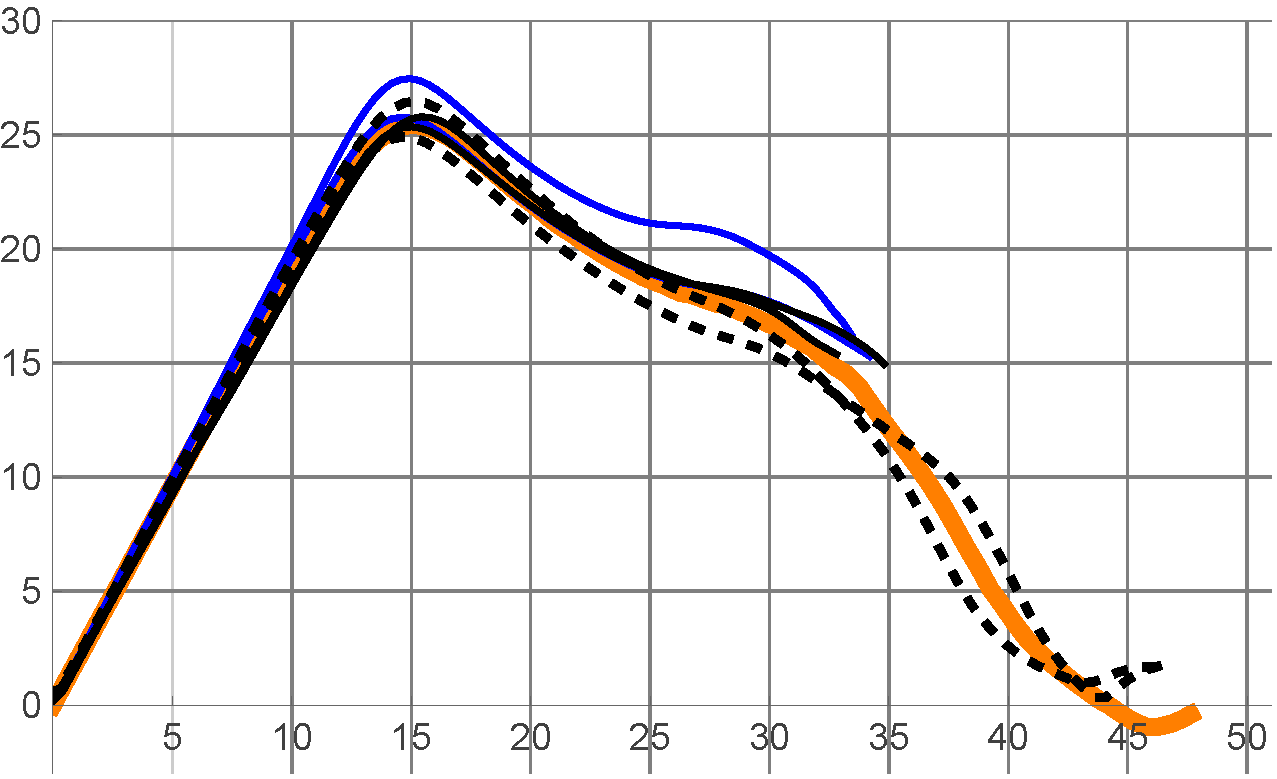
\includegraphics[width=0.95\linewidth]{figures/profiles.pdf}}
		\put(35,12){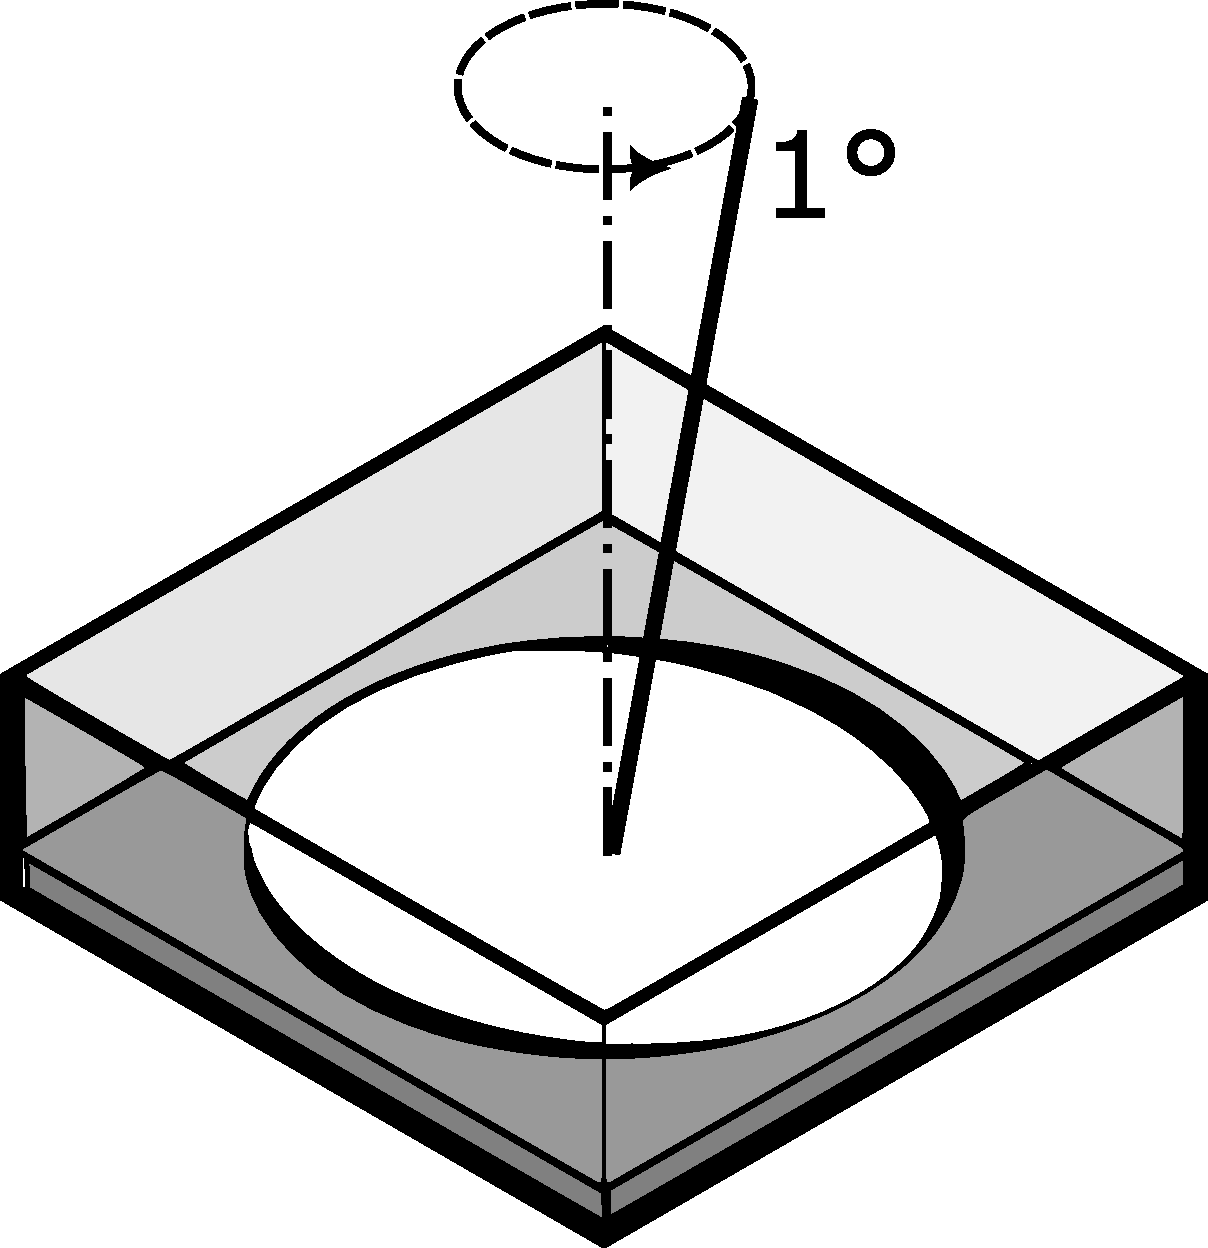
\includegraphics[width=0.35\linewidth]{figures/scheme_nut.pdf}}
	\end{picture}
	% TODO: [Velocity data] Specify the plotted r and U units, the rotation rate,
	% and the averaging/uncertainty estimates. For r>35 cm, describe the angular
	% weighting and how the partial-circle average is used as an axisymmetric U(r).
	\caption{Radial profiles of the mean azimuthal velocity measured in the experiment. The thick orange line shows the azimuthal average; at radii $r>35\,\text{cm}$, the average is taken only over the portion of the circle within the basin. The solid blue and black lines show the velocity profiles along the two directions parallel to the sidewalls. The dashed line shows the profile along a diagonal. Inset: schematic of the experimental setup.}
	\label{fig:U-profiles}
\end{figure}

% TODO: [Measurement resolution] Describe the waiting time used to establish a
% steady mean flow, PIV spatial resolution and velocity uncertainty, and temporal
% filtering. Explain the transformation/Fourier projection from v^x,v^y to the
% complex azimuthal wave amplitudes at fixed m and frequency used below.
The horizontal components of the fluid velocity at the free surface, $v^x$ and $v^y$, are measured using particle image velocimetry (PIV). Polyamide PA-12 particles are scattered over the free surface. A camera mounted above the center of the basin records the horizontal motion of the particles. For each experiment, a video of duration $T=175\,\text{s}$ is recorded at a frame rate of $24\,\text{Hz}$.

% TODO: [Frequency convention] Distinguish disk rotation frequency in Hz from
% angular velocity in rad/s. The later exp(-i*omega*t), U/r, and Doppler shift
% require angular frequencies; state every 2*pi conversion used in text and figures.
% Clarify whether 0.3 Hz is a rounded upper endpoint for the selected 0.31 Hz run.
% TODO: [Flow regime] Collapse of U(r) after normalization does not establish
% laminar flow or linear instantaneous dynamics. Provide fluctuation/stability
% evidence and reconcile the claim with the turbulent sidewall layer below;
% yang2019axisymmetric also reports unsteady 3D high-Re flows with similar means.
Ten approximately uniformly spaced angular velocities in the range $0.024$--$0.3\,\text{Hz}$ were tested. In each case, the radial profile of the azimuthal velocity $U$ was measured in a polar coordinate system $\{r,\varphi\}$ centered on the basin. All profiles coincided after their amplitudes were normalized by the disk rotation speed. This indicates that the mean flow responds linearly and can be considered laminar. The profiles $U(r)$, both averaged over the azimuthal angle $\varphi$ and measured along selected directions, are plotted in Figure~\ref{fig:U-profiles}. In what follows, we consider only the experiment with the highest disk rotation speed, $\Omega \approx 0.31\,\text{Hz}$. For pure water, the Reynolds number characterizing the mean flow is $\mathrm{Re} = 40 000$, using a characteristic velocity of $25\,\text{cm}/\text{s}$ and a characteristic length of $15\,\text{cm}$.

% TODO: [Rotation/profile comparison] Is lim_{r->0} U/r measured to equal the
% disk angular velocity Omega, or is this an approximation/different parameter?
% State the nondimensionalization and matched depth/radius and disk/basin ratios
% used when importing the mean-flow properties of yang2019axisymmetric.
Our setup is similar to that studied in Ref.~\cite{yang2019axisymmetric}, differing only in the basin geometry: our basin is square, whereas that in Ref.~\cite{yang2019axisymmetric} is cylindrical. Despite this difference, the radial profiles $U(r)$ agree well. In particular, the core in which the fluid undergoes solid-body rotation has a radius of \hbox{$\approx 14\,\text{cm}$} in our setup, approximately half the disk radius. This ratio is consistent with the $U(r)$ profiles in Ref.~\cite{yang2019axisymmetric}, where the position of the maximum of $U(r)$ was found to depend on the aspect ratio $D/R$. The angular velocity $U/r$ reaches its maximum $\Omega$ at the center and decreases slightly toward the core edge, also consistent with the observations in Ref.~\cite{yang2019axisymmetric}. We did not measure the vertical profile of the azimuthal velocity, but we expect it to be uniform except within the thin boundary layer near the bottom, based on the measurements in Ref.~\cite{yang2019axisymmetric}.

The deformation of the fluid surface due to centrifugal forces is relatively small. To estimate the difference in surface elevation between the edge and the center, we use Euler's equation,
\begin{equation}\label{eq:N-S}
% TODO: [Pressure/gravity] Reconcile this equation with the definition immediately
% below. If P_total=P-gz is physical pressure per unit density, Euler's equation
% also contains -g*e_z; if gravity is absorbed, its right-hand side is -grad P.
% Define the pressure variables consistently before linearizing the equations.
	\partial_t {\bm v} + ({\bm v}\nabla){\bm v} = - \nabla P_{\mathrm{total}},
\end{equation}
where the water density is set to unity and the physical pressure is $P_{\mathrm{total}} = P - gz$. For an axisymmetric, steady flow, the radial component of Euler's equation (\ref{eq:N-S}) is
\begin{equation}
	\partial_r P - U^2/r = 0.
\end{equation}
% TODO: [Reference surface/volume] Define z=0 as the volume-equivalent still-water
% level if the integral of H is to vanish. The radial volume condition below is
% for a circular domain; the square basin requires its actual area weighting.
% State explicitly whether this is a cylindrical approximation to the experiment.
The boundary condition at the fluid surface $z=H(r)$ is $P = gH$, since the physical pressure $P_{\mathrm{total}} = 0$ after subtracting the constant atmospheric pressure. For a given $U(r)$, the pressure solution gives
\begin{equation}
	H(r) = H(0)
	+ \frac{1}{g}\int\limits_0^r \mathrm{d}r^\prime \frac{U^2(r^\prime)}{r^\prime},
	\qquad
	\int\limits_0^R Hr\mathrm{d}r = 0.
\end{equation}
% TODO: [Effective radius] Justify R=47 cm and state whether the same value is
% used for every theoretical mode. Distinguish it from the 30 cm disk radius,
% 35 cm basin half-width, and approximately 49.5 cm center-to-corner distance;
% quantify the sensitivity of wall-reaching modes to this choice and to U(r).
The integral condition expresses conservation of the total fluid volume. For the profile shown in Figure~\ref{fig:U-profiles}, the elevation difference is $H(R) - H(0) \approx 8\,\text{mm}$, assuming $R=47\,\text{cm}$. This is approximately one-twelfth of the water depth~$D$.

% TODO: [Neglected advection] Specify where/how the ratio 0.1 is evaluated and
% estimate k_r*U^r relative to the intrinsic wave frequency, together with the
% effects of mean-flow gradients and nonaxisymmetry. A velocity ratio alone does
% not bound frequency shifts or coupling between azimuthal Fourier components.
The boundary layer generates secondary flows in the radial and vertical directions \cite{yang2019axisymmetric}. These flows are weak compared with the azimuthal flow. In our setup, the measured mean radial velocity at the surface is also relatively small, $U^r/U^\varphi\sim 0.1$. The radial flow is not axisymmetric but instead follows the symmetry of the square basin.

% TODO: [Forcing harmonics] Give the temporal/azimuthal spectrum of the disk forcing.
% A steady linear wave operator driven only by a sinusoidal tilt at Omega does not
% generate higher temporal harmonics. Identify nonsinusoidal forcing, time-periodic
% coefficients, or nonlinear generation, and separate that process from wave response.
% TODO: [Linearity/linewidth] Narrow forced peaks do not establish linearity:
% a nonlinear periodic response can also have narrow harmonics. Give
% wave steepness or amplitude-scaling evidence, spectral resolution/windowing, and
% a separate damping/resonance-width estimate if linewidth is used dynamically.
The disk rotation also excites waves because the disk plane is tilted by $1^\circ$ from the horizontal, whereas the rotation axis is aligned with the vertical to greater precision. The rotating disk thus periodically perturbs the fluid motion. The measured frequency spectrum of the velocity field shows an appreciable response only at integer multiples of $\Omega$; see Figure~\ref{fig:spectrum}. The peaks are narrow, so nonlinear peak broadening can be neglected and the system can be assumed to be in the linear-response regime. The peak amplitude does not vary monotonically with frequency. This is because the stronger overtones of $\Omega$ lie closer to the resonant modes of the system than the weaker overtones, as discussed below.


\begin{figure}[t]
	\begin{picture}(230,140)
		\put(10,0){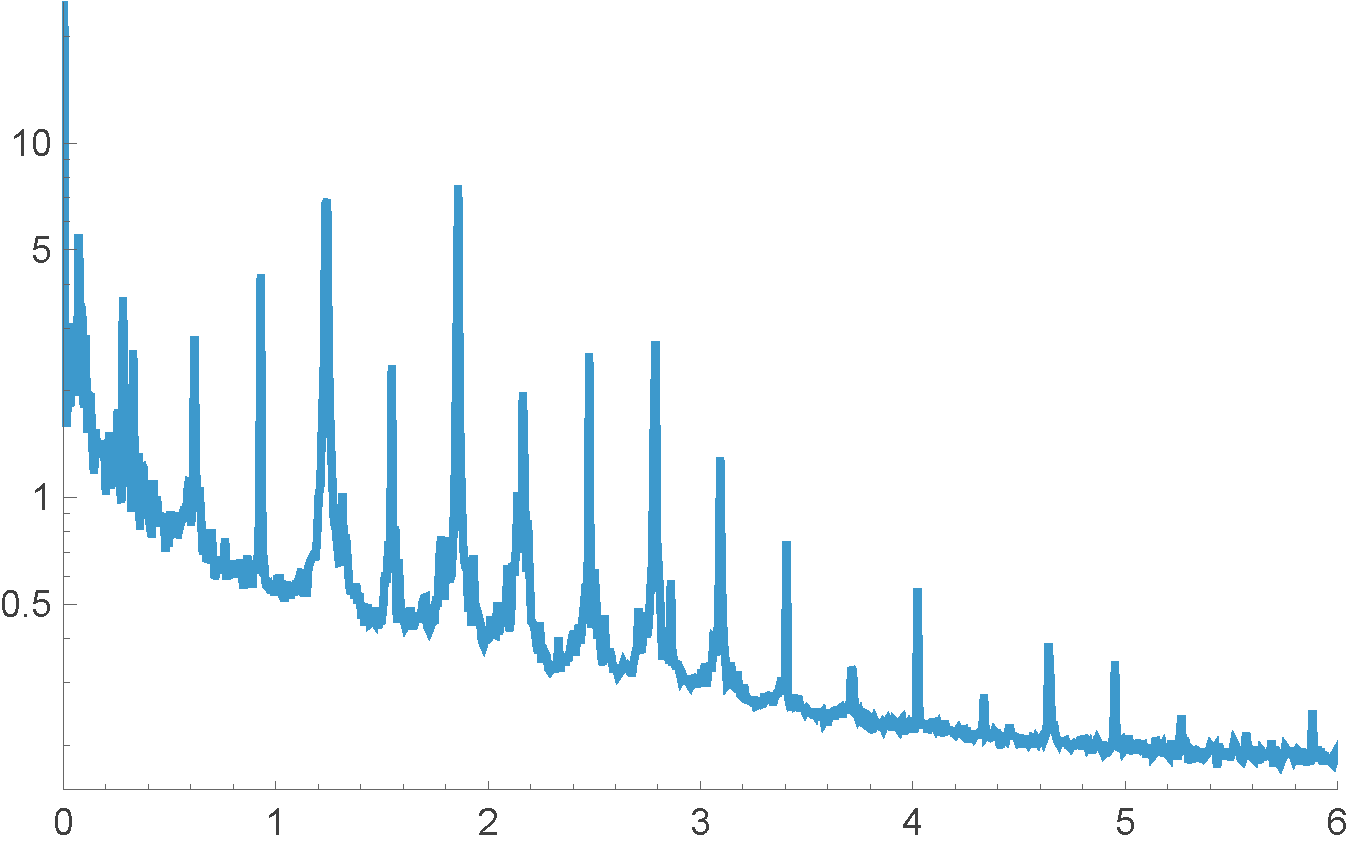
\includegraphics[width=0.85\linewidth]{figures/spectrum.pdf}}
		\put(225,10){\vbox{\hbox{{\large$\omega,$}} \hbox{Hz}}}
		\put(0,55){\rotatebox{90}{{\large $E_\omega$}, arb. u.}}
	\end{picture}
	% TODO: [Spectral definition] Define v_omega, mean subtraction, one-/two-sided
	% normalization, and whether E_omega is a density or a squared Fourier amplitude.
	% A full 175 s record has nominal resolution 1/T approximately 0.0057 Hz; specify
	% any shorter windows. This surface horizontal kinetic-energy measure is not
	% automatically total wave energy, including vertical motion and surface elevation.
	\caption{Energy spectrum of the horizontal motion at the surface, $E_\omega = (\langle|v^x_\omega|^2\rangle + \langle |v^y_\omega|^2\rangle)/2$, where angle brackets denote averaging over the surface. The peaks occur at integer multiples of the angular velocity $\Omega$ of the disk.}
	\label{fig:spectrum}
\end{figure}




\section{Theory}
\label{sec:theory}

% TODO: [Bottom-layer approximation] Estimate penetration into the bottom shear
% layer for the actual modes, not just a characteristic wavelength. kD >= 1 does
% not imply negligible bottom motion; clarify how the finite-depth calculation
% below supports neglecting bottom-layer shear and direct bottom forcing.
We assume an axisymmetric basin of radius $R$ and depth $D$. We introduce cylindrical coordinates $\{r,\varphi,z\}$, with $z=0$ at the unperturbed fluid surface. The ring current is steady and axisymmetric, ${\bm U} = U(r) {\textbf e}_\varphi$, where ${\textbf e}_\varphi$ is the azimuthal unit vector. We decompose the total fluid velocity ${\bm v}$ into the current velocity and the wave velocity ${\bm u}$, ${\bm v} = {\bm U}+{\bm u}$. Because we are primarily interested in waves with a relatively short characteristic wavelength $\lambda$, $\lambda/2\pi \lesssim D$, we neglect the vertical variation of the mean azimuthal velocity $U^\varphi$ within the boundary layer near the bottom. We also neglect the small radial and vertical components of the mean flow.

% TODO: [Linearization] Define p explicitly as the wave perturbation of the chosen
% reduced pressure. State the small-amplitude ordering and justify neglecting
% viscous/turbulent damping for eigenfrequencies while discussing its possible
% importance for forced amplitudes and detectability.
Euler's equation (\ref{eq:N-S}), linearized with respect to the surface wave amplitude, and the continuity equation are
\begin{equation}\label{linearized:001}
	\partial_t {\bm u}
	+
	({\bm U} \nabla) {\bm u}
	+
	({\bm u} \nabla){\bm U}
	=
	-\nabla p,
	\qquad
	\mathop{\mathrm{div}}{\bm u} = 0.
\end{equation}
% TODO: [Eigenproblem versus forcing] State that the homogeneous bottom condition
% defines free eigenmodes, not the response to the moving tilted disk. A prediction
% of excitation requires the inhomogeneous boundary forcing and its modal overlaps.
The boundary conditions are $u^z = 0$ at the bottom and $u^r=0$ at the sidewall. We write the free surface as $z = H + h$, where $h$ is the wave-induced displacement. The kinematic boundary condition at the free surface is
\begin{equation}\label{BC:kinematic}
% TODO: [Equilibrium surface slope] Linearization about z=H(r) gives
% (partial_t + (U/r)*partial_phi)h = u^z - H'(r)*u^r, evaluated at z=H(r).
% State the additional approximation that removes H'*u^r and moves evaluation
% to z=0. Check surface slope and k*|H|; small H/D alone does not justify this
% replacement for all short waves or preserve exact separation of variables.
	\partial_t h + \big({\bm U}\vert_{z=0} \nabla\big) h
	=
	u^z\big\vert_{z=0}.
\end{equation}
The dynamic boundary condition is
\begin{equation}\label{BC:dynamic}
	p + h \partial_z P = gh.
\end{equation}
% TODO: [Vertical pressure balance] Derive partial_z P=0 using the reduced-pressure
% convention and the steady mean vertical momentum balance with negligible
% meridional flow; vertical uniformity of U alone is not the full justification.
The term $h\partial_z P$ vanishes because the mean flow is assumed to be vertically uniform. We neglect capillary effects because the characteristic wavelength lies in the gravity-wave regime.

% TODO: [Wave/sign convention] State omega>0 and the orientation of phi, and explain
% whether plotted positive m and U are magnitudes when the theory requires mU<0.
% Specify whether "against the current" refers to phase or group/energy propagation.
% Also clarify that upper/lower velocity indices denote the same physical components
% in an orthonormal cylindrical basis, rather than covariant/contravariant components.
We consider a mode with frequency $\omega$ and azimuthal mode number $m$, so that all wave fields $p, u^r, u^\varphi, u^z$ are proportional to $\exp(im\varphi - i \omega t)$. The components of Euler's equation (\ref{linearized:001}) are then
\begin{equation}\label{u_r_init}
	\begin{aligned}
		-i\widetilde \omega u_r - 2(U/r)u_\varphi & = -\partial_r p,
		\\[5pt]
		-i\widetilde \omega u_\varphi +
		\big(2(U/r) + \Sigma\big) u_r             &
		= -i(m/r)\,p,
		\\[5pt]
		-i\widetilde \omega u_z                   & = -\partial_z p,
	\end{aligned}
\end{equation}
where $\widetilde \omega(r) = \omega - m U/r$ is the Doppler-shifted frequency and $\Sigma = r \partial_r (U/r)$ is the local shear rate of the mean flow. The continuity equation is
\begin{equation}\label{continuity-eq}
	\frac{\partial_r(r u_r)}{r} +\frac{im u_\varphi}{r} + \partial_z u_z
	= 0.
\end{equation}
The linearized Euler equations (\ref{u_r_init}) express all velocity components in terms of the pressure $p$:
% TODO: [Algebra: horizontal signs] Recheck this matrix inversion with the stated
% exp(-i*omega*t) convention and Lambda. At U=0, the momentum equations require
% u_r=-i*partial_r p/omega and u_phi=m*p/(r*omega), whereas both printed horizontal
% expressions give the opposite signs. The printed u_z sign is consistent.
\begin{equation}
	\begin{aligned}
		u_z =     & \,-\frac{i}{\widetilde\omega }\,\partial_z p,
		\qquad
		u_r = \frac{i}{\Lambda}
		\left(
		\widetilde\omega\,\partial_r - \frac{2mU}{r^2}
		\right)p,
		\\[5pt]
		u_\varphi & = \frac{1}{\Lambda }\, \left(
		\left(\frac{2U}{r}+\Sigma\right)\partial_r -\frac{m\widetilde \omega}{r}
		\right)p.
	\end{aligned}
\end{equation}

Substituting these expressions into the continuity equation (\ref{continuity-eq}) gives
% TODO: [Elimination consistency] This pressure equation agrees with continuity
% when both horizontal velocity expressions above have their signs reversed,
% not when they are used as printed. Check the derivation and the implementation
% together; do not change the pressure operator merely to match a transcription error.
\begin{equation}\label{p_eq_init}
	\frac{\widetilde\omega^2}{r}\left(\partial_r
	\frac{r}{\Lambda}\partial_r
	-
	\frac{m(m+2\Sigma/\widetilde \omega)}{r\Lambda}
	+
	\frac{2mU\Lambda^\prime}{r\widetilde \omega \Lambda^2}
	\right)p
	+
	\partial_z^2 p = 0,
\end{equation}
% TODO: singularity ?= instability, singularity == critical layer
% TODO: [Singularities] Distinguish tilde_omega=0 (a corotation/critical layer)
% from Lambda=0 (an inertial/epicyclic resonance). Neither condition by itself
% proves temporal instability; a stability claim requires an appropriate analysis.
% TODO: [Regularity range] Quantify "omega sufficiently large" or verify
% tilde_omega and Lambda stay bounded away from zero throughout each calculated
% mode's domain. Treat the coordinate singularity at r=0 with a regularity condition.
% TODO: [Base-flow stability] Assess kappa^2=2(U/r)(2U/r+Sigma)
% =r^(-3)*d[(rU)^2]/dr. If (rU)^2 decreases outward toward a wall where U=0,
% kappa^2 is negative somewhere, raising centrifugal-stability questions for an
% inviscid laminar base state. Explain relevant stabilization or the mean-flow model.
% TODO: [Continuous spectrum/nonlinearity] Show the m-resolved continuous spectrum
% and reconcile it with the earlier description of appreciable response only at
% harmonics. Quantify "moderate" and justify negligible nonlinear coupling by
% amplitudes/time scales rather than the spectrum's appearance alone.
where $\Lambda = \widetilde \omega^2 - 2(U/r)(2U/r+\Sigma)$ and the prime denotes differentiation with respect to the radial coordinate $r$. We consider only waves propagating against the current, so $mU<0$, with $\omega$ sufficiently large. Under these conditions, neither the shifted frequency $\widetilde\omega$ nor $\Lambda$ vanishes, and equation (\ref{p_eq_init}) is regular everywhere. A singularity would correspond to an instability. Experimentally, we observe a continuous spectrum in the range $mU>0$. Its amplitude is moderate, allowing us to neglect nonlinear interactions between waves with $mU<0$ and $mU>0$.

% TODO: \partial_r p = 0 != u_r = 0 on sidewall
% TODO: [Sidewall condition] For nonzero Lambda, impermeability requires
% tilde_omega*partial_r p - (2*m*U/r^2)*p=0 at r=R. The stated Neumann condition
% follows if U(R)=0 (or another stated special case). Specify the imposed endpoint
% of U(r) and verify that the radial eigenfunctions use the appropriate condition.
The boundary conditions are $\partial_z p =0$ at the bottom and $\partial_rp=0$ at the sidewall. At the free surface, the kinematic boundary condition (\ref{BC:kinematic}) becomes $-i\widetilde\omega h = u^z $. Combining this condition with the dynamic boundary condition (\ref{BC:dynamic}) and the vertical component of Euler's equation (\ref{u_r_init}) gives the boundary condition for $p$ at $z=0$:
\begin{equation}\label{BC-for-p:free-surafec}
	\big( g \partial_z - \widetilde\omega^2\big) p
	=
	0.
\end{equation}

% TODO: [Validation limit] Verify that the numerical method recovers the regular
% Bessel modes with omega^2=g*k*tanh(kD) at U=0; this also tests the signs and
% the missing-factor issue in the surface operator below.
In the absence of a mean flow, the wave equation (\ref{p_eq_init}) reduces, after separation of variables, to Bessel's equation of order $m$. Assuming $\partial_z^2 p = k^2 p$, we obtain $p_k = {\mathrm J}_m(kr)\cosh(k(z+D))$. The allowed wavenumbers $k$ are determined by the sidewall boundary condition, ${\mathrm J}^\prime_m(kR) = 0$. The free-surface boundary condition (\ref{BC-for-p:free-surafec}) determines the wave frequency $\omega$.

In the presence of a mean flow, equation (\ref{p_eq_init}), together with the conditions at the rigid boundaries, can still be solved by separation of variables. However, the free-surface boundary condition (\ref{BC-for-p:free-surafec}) now depends on the radial coordinate, so the full problem does not admit separation of variables.

% TODO: [Reproducible model input] Provide the actual U(r) data/fit, its smoothing
% and endpoint treatment, and R,D used in the solver. The coefficients involve
% derivatives of U, including those in Lambda', so the plotted curve alone is
% insufficient to reproduce eigenfrequencies, turning points, or uncertainty.
% TODO: [Radial eigenproblem] Specify the radial ODE, central regularity
% (for smooth solid-body behavior, p proportional to r^|m|), eigenfunction
% normalization, and ordering of k_i. Make explicit that k_i and F_i depend on
% the trial omega and m and must be determined consistently during root finding.
% TODO: [Surface operator: dimensions] For F_i proportional to cosh(k_i(z+D)),
% (partial_z F_i)/F_i at z=0 is k_i*tanh(k_iD). Check the missing k_i multiplying
% g in B(k_i): g*tanh(k_iD) and tilde_omega^2 have different dimensions.
% Moreover B_i depends on r through tilde_omega(r); it is not a scalar eigenvalue
% and its radial dependence must remain inside the projection integral.
We solve the full problem numerically. We determine the first $N$ eigenfunctions ${\mathcal F}_i(r,z)$ and wavenumbers $k_i$ of equation (\ref{p_eq_init}), subject to the bottom and sidewall boundary conditions. The action of the linear operator $\hat {\mathcal B} = g \partial_z - \widetilde\omega^2$ from (\ref{BC-for-p:free-surafec}) on an eigenfunction at the surface is $\hat {\mathcal B} {\mathcal F}_i = B(k_i){\mathcal F}_i$, where $B(k_i) = g\tanh(k_iD) - \widetilde\omega^2$. We then construct an orthonormal basis ${\mathcal J}_i(r)$ from the first $N$ solutions of (\ref{p_eq_init}) for $U=0$, evaluated at the surface. The inner product uses the integration measure $r\mathrm{d}r$ for the radial coordinate $r$. We expand the solution as
\begin{equation}
	p = \sum_{i=1}^N A_i {\mathcal F}_i.
\end{equation}
In this basis, the free-surface boundary condition (\ref{BC-for-p:free-surafec}) becomes
\begin{equation}
	\sum_{i=1}^N B_{ji}A_i = 0,
	\qquad
	B_{ji}
	=
	\big\langle {\mathcal J}_j \big\vert B(k_i)\, {\mathcal F}_i(z=0)\big\rangle.
\end{equation}
% TODO: finite N != only shift of solution
% TODO: [Convergence] Reality of the determinant does not bound truncation errors
% or exclude missed/spurious roots. Show convergence of frequencies and profiles
% as N increases beyond 15, and report the free-surface boundary residual and
% numerical root tolerance; clarify whether complex-frequency modes were excluded.
A nontrivial solution exists only if the matrix is singular, $\mathop{\mathrm{det}}|B_{ij}| = 0$. The determinant is a real function of the frequency $\omega$, so errors due to the finite cutoff $N$ in the sums only slightly shift a solution. For our purposes, $N=15$ was sufficient. We denote each solution by $\omega_{m,n}$, where the positive integer $n$ increases with eigenfrequency. Once the frequency $\omega_{m,n}$ is found, the coefficients $A_i$ are given by an eigenvector of the matrix~$B_{ji}$ with zero eigenvalue.

\begin{figure}[t]
	\centering
	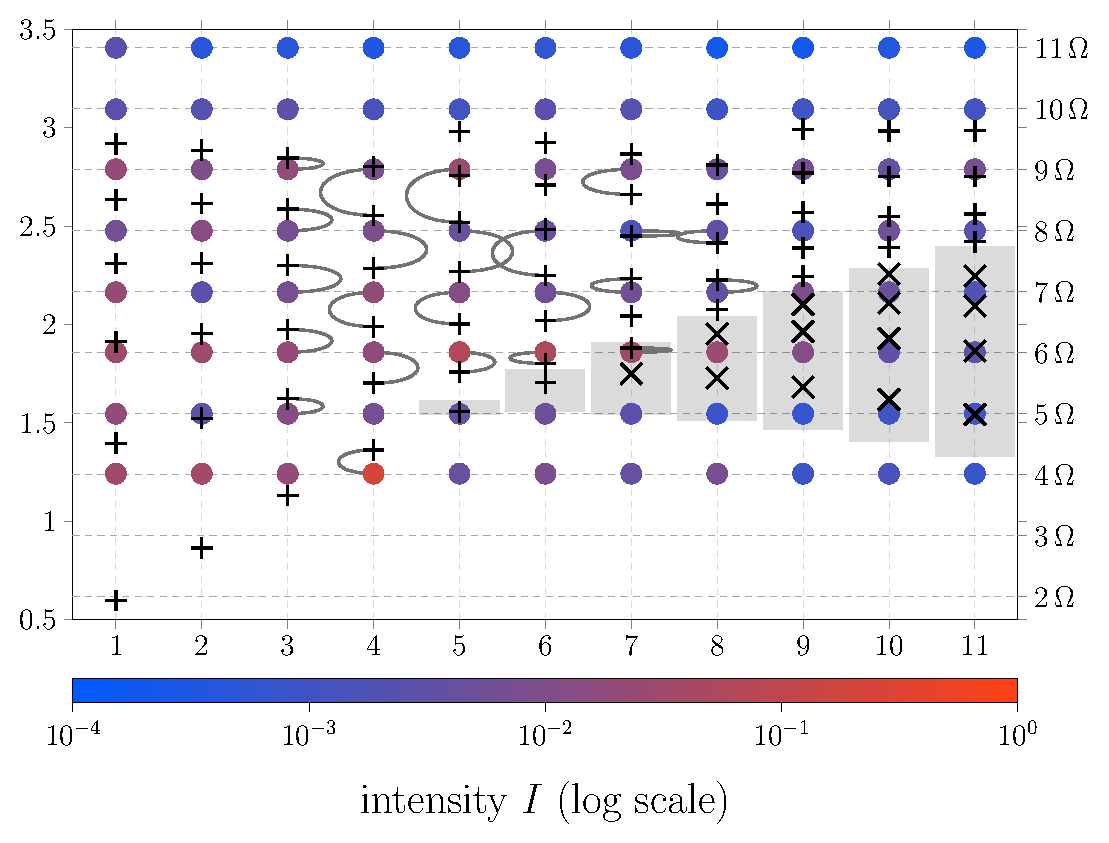
\includegraphics[width=1.0\linewidth]{figures/map.pdf}
	% TODO: [Intensity/energy] Define the plotted I, its units or normalization,
	% radial/angular integration domain, and its relation to E_omega and "mean energy".
	% Explain whether the same normalization permits comparisons across m and frequency.
	\caption{Map of eigenmodes in the plane of azimuthal mode number $m$ (horizontal axis) and frequency in hertz (vertical axis). Plus signs and crosses denote theoretically calculated delocalized and trapped eigenmodes, respectively. Gray regions show WKB estimates of the frequency bands in which modes are trapped by the mean flow. Filled circles represent experimentally measured wave fields, with colors indicating the mean energy stored in the fields. Curved lines connect theoretical modes to experimental wave fields with corresponding spatial profiles.}
	\label{fig:map}
\end{figure}


% TODO: [Nodal indexing] Justify identifying frequency order n with n-1 interior
% zeros of u_phi in this frequency-dependent, nonseparable problem; distinguish
% an observed numerical rule from a nodal theorem. For |m|=1, regular p~r gives
% finite, generally nonzero horizontal velocity at r=0, already in the U=0 limit,
% so the assertion that u_phi vanishes there needs qualification.
The results of the numerical procedure are shown in Figure~\ref{fig:map}. Plus signs and crosses in the $m$-$\omega$ plane denote the calculated eigenmodes. These modes lie along approximately horizontal curves. Each curve corresponds to a fixed radial mode number $n$, which counts the radial half-waves. The lowest-frequency modes at fixed $m$ have $n=1$. In these modes, the velocity component $u_\varphi$ vanishes only at $r=0$. In other modes, $u_\varphi$ has $n-1$ additional zeros within the interval $r<R$. Examples of radial eigenmode profiles are plotted in Figure~\ref{fig:wave-theory}.

% TODO: [Deep-water bound] Deep water requires kD>>1, not merely kD>1.
% At lambda=2*pi*D, tanh(kD)=0.762 and 1/cosh(kD)=0.648; finite-depth effects
% and bottom motion are not small. Give an accuracy criterion and check local kD
% over each mode, or quantify the difference from finite-depth WKB estimates.
% TODO: [Capillary bound] The group-velocity minimum is not a criterion for
% negligible surface tension. Check sigma*k^2/(rho*g)<<1 for the relevant modes;
% at lambda=4 cm it is about 0.18 using typical clean-water sigma=0.073 N/m,
% rho=1000 kg/m^3, and g=9.81 m/s^2 (illustrative values, not measurements here).
% TODO: [WKB ordering] State the short-wavelength/slow-variation conditions and
% the ordering of |U/r| and |Sigma| relative to |tilde_omega| that permits the
% gravity-only local dispersion law. Explain the turning-point treatment and
% assess its accuracy for the low radial mode numbers used to classify trapping.
We consider waves in the deep-water regime for which capillary effects remain negligible. The characteristic wavelength $\lambda$ must therefore lie in the interval $4\,\text{cm} < \lambda < 60\,\text{cm}$, where the lower bound corresponds to the minimum group velocity of capillary-gravity waves and the upper bound is $2\pi D$. To estimate the radial dependence of the wave field, we use the WKB approximation in the short-wavelength limit. The local dispersion relation is $\widetilde \omega^2  = gk$. The squared wavenumber is $k^2 = m^2/r^2 + k_r^2$, where $k_r$ is the radial wavenumber. Thus, the relation
\begin{equation}\label{eq:kr}
	k_r^2 (r;\omega,m)
	=
	\frac{\widetilde\omega^4}{g^2} - \frac{m^2}{r^2}
\end{equation}
% TODO: [Turning-point interpretation] Distinguish the wave's angular-momentum
% barrier m^2/r^2, which remains at U=0, from the centrifugal force of the mean
% current. State the parameter assumptions ensuring the claimed number of roots.
% TODO: [Trapping criterion] Require turning points within the physical domain
% and specify a radial action/quantization condition: well width as well as depth
% matters. Check for a third turning point and a propagating outer region before
% the sidewall, and quantify barrier attenuation. Define how trapped versus
% delocalized modes are classified from the numerical fields in a finite basin.
describes the radial oscillations of the mode velocity field. Toward the vortex center, $k_r$ vanishes at some $r=r_l$ because of the centrifugal force represented by the last term in (\ref{eq:kr}). If the ring current is absent or sufficiently weak, $k_r$ remains real for all $r>r_l$. The wave therefore reaches the sidewall and is reflected by it. If the current is sufficiently strong, $k_r$ vanishes again at some $r_r > r_l$. In this case, the wave is expected to be trapped (i.e., localized) within the ring current. The light gray regions in Figure~\ref{fig:map} indicate where the point $r_r$ exists. However, the potential well must be sufficiently deep for localization to occur, so the gray regions slightly overestimate the range in which localized modes exist. The modes denoted by crosses are indeed localized, with amplitudes that decay exponentially toward the sidewall.

\begin{figure}[t]
	\begin{picture}(250,150)
		\put(0,-10){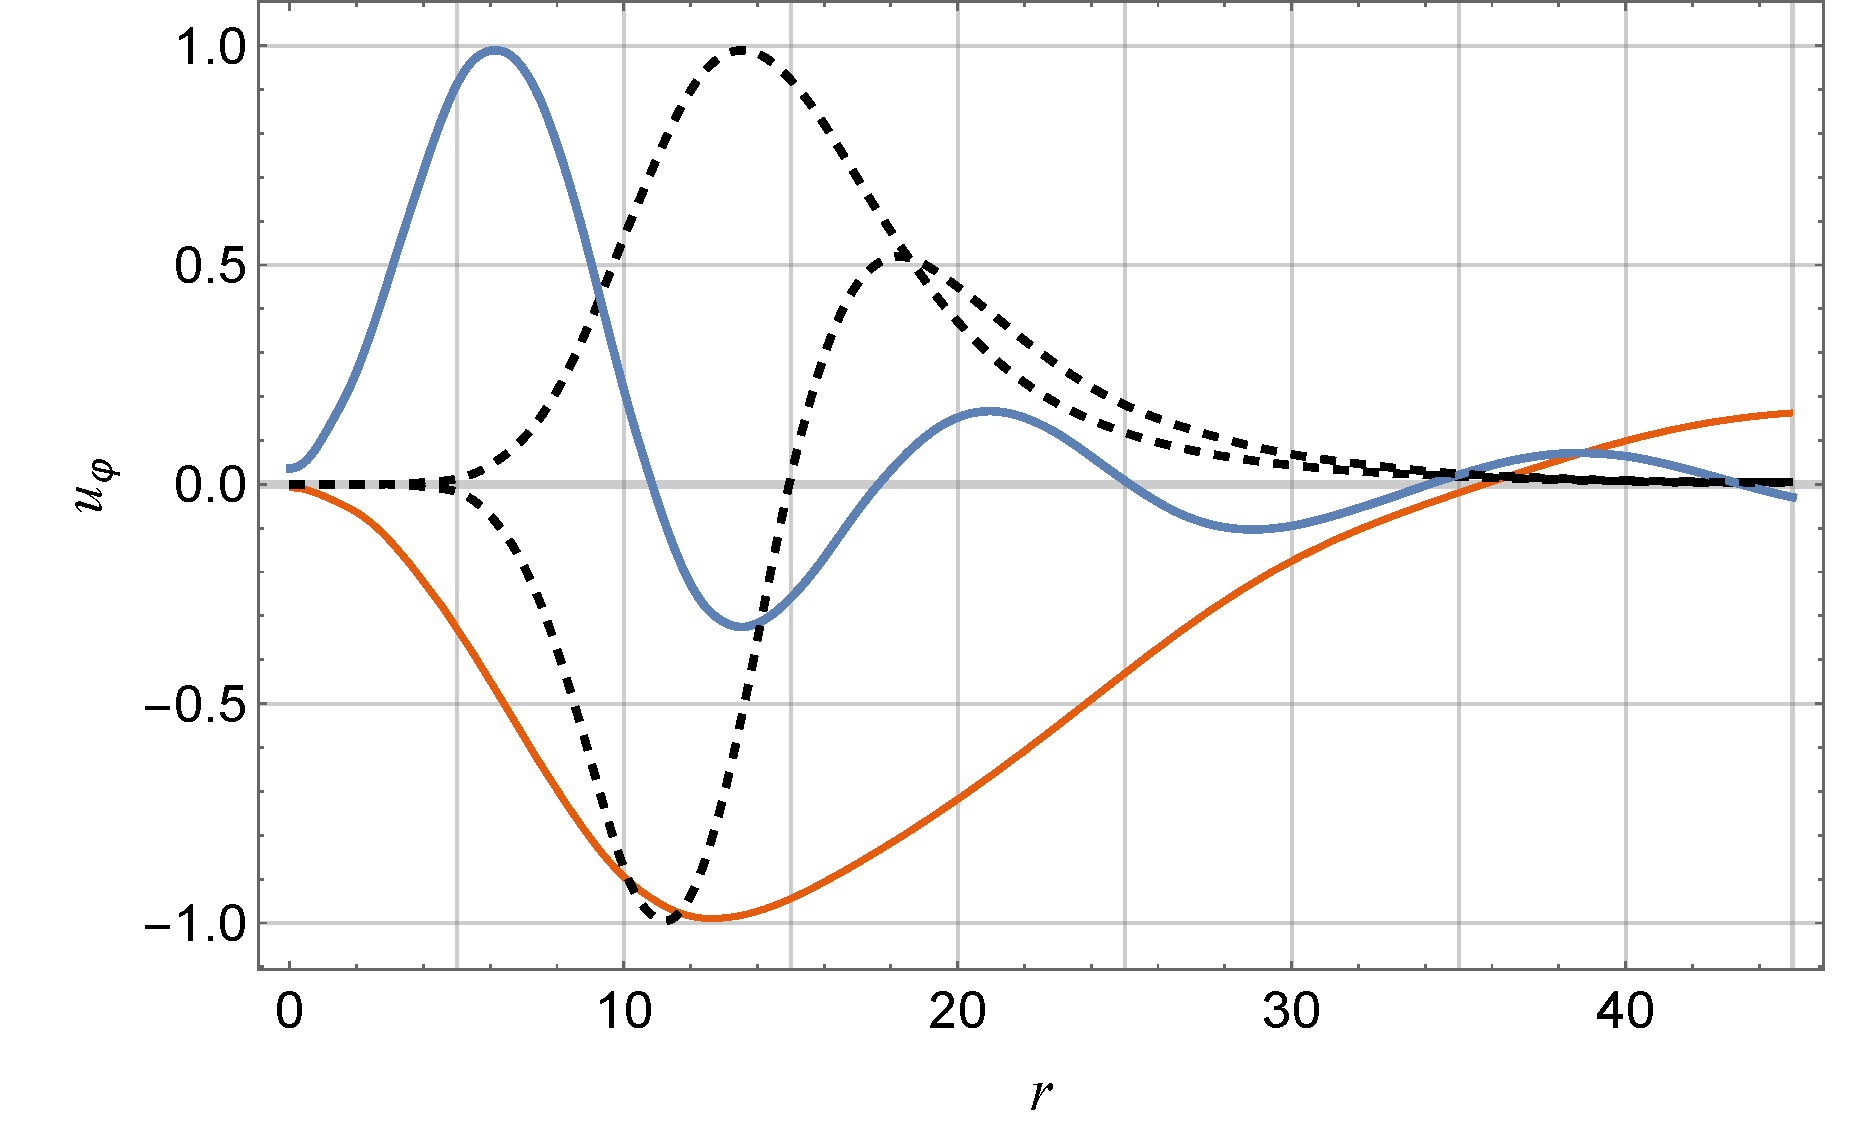
\includegraphics[width=1.0\linewidth]{figures/wave-theory.pdf}}
		\put(53,100){\rotatebox{70}{\scriptsize $(3,\,6)$}}
		\put(115,120){$(8,\,1)$}
		\put(105,45){$(10,\,2)$}
		\put(130,30){\rotatebox{33}{$(3,\,2)$}}
	\end{picture}
	% TODO: [Mode-profile definition] Specify the evaluation height, radial units,
	% and eigenfunction amplitude/phase normalization; free eigenmodes have arbitrary
	% scale and their signed profiles are not directly comparable without a convention.
	\caption{Examples of radial profiles of the azimuthal wave velocity $u_\varphi$. The labels give the mode numbers $(m,\,n)$. Dashed curves show modes that can be considered radially localized by the mean flow.}
	\label{fig:wave-theory}
\end{figure}

Figure~\ref{fig:wave-theory} shows examples of radial mode profiles in terms of the azimuthal velocity component $u_\varphi$. Dashed curves denote modes that can be considered radially localized by the mean flow.

\begin{figure}[t]
	\centering
	\begin{picture}(250,210)
		\put(1.9,145){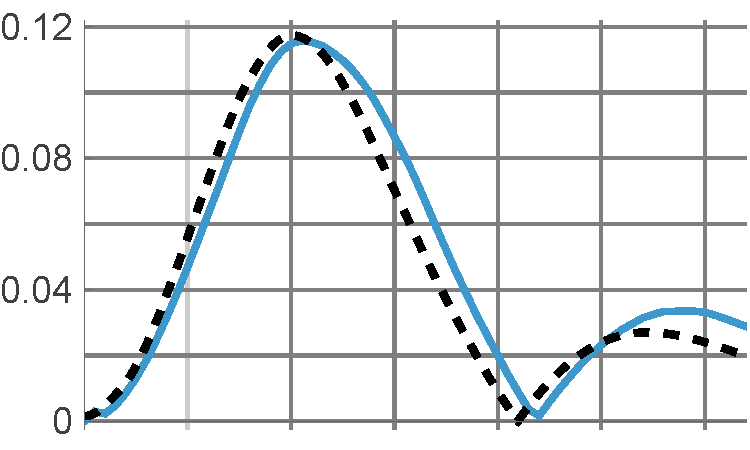
\includegraphics[width=0.447\linewidth]{figures/3-3.pdf}}
		\put(70,190){$6\Omega, \ \ (3,\,3)$}
		\put(18,195){\textbf{a)}}

		\put(130,145){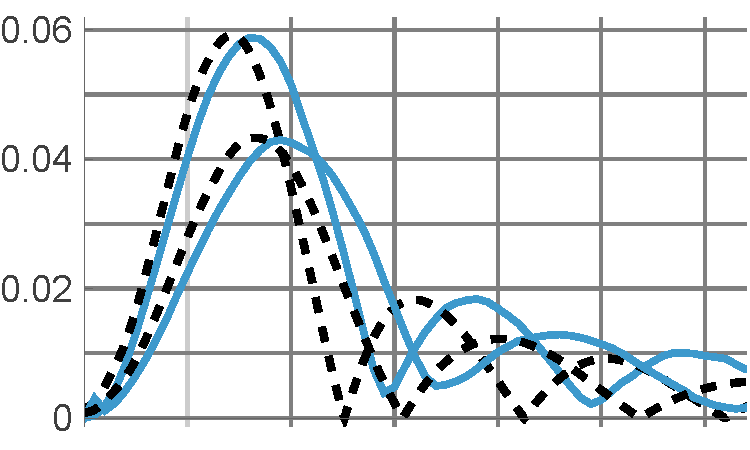
\includegraphics[width=0.45\linewidth]{figures/3-4, 3-5.pdf}}
		\put(193,200){$7\Omega, \ \ (3,\,4)$}
		\put(193,185){$8\Omega, \ \ (3,\,5)$}
		\put(225,166){\textbf{b)}}

		\put(2.8,73){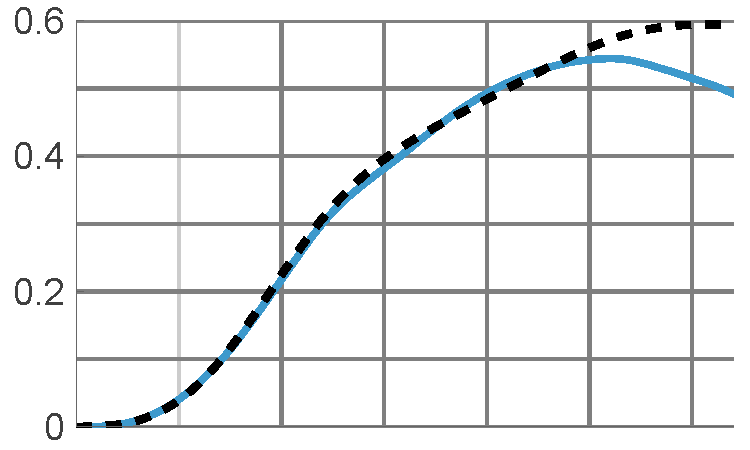
\includegraphics[width=0.45\linewidth]{figures/4-1.pdf}}
		\put(70,105){$4\Omega, \ \ (4,\,1)$}
		\put(18,115){\textbf{c)}}

		\put(130,72.5){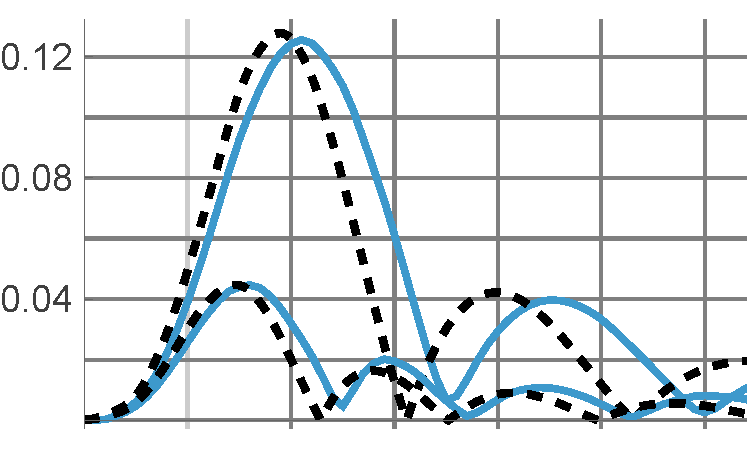
\includegraphics[width=0.45\linewidth]{figures/4-4, 4-6.pdf}}
		% TODO: [Cross-figure mode assignment] Reconcile these (4,4) at 7*Omega and
		% (4,6) at 9*Omega labels with map.tex/ArcData: the corresponding fields are
		% connected to (4,3) and (4,5), respectively. Verify the actual calculated
		% profiles and radial indexing before changing either figure's assignments.
		\put(193,120){$7\Omega, \ \ (4,\,4)$}
		\put(193,105){$9\Omega, \ \ (4,\,6)$}
		\put(145,120){\textbf{d)}}

		\put(0,0){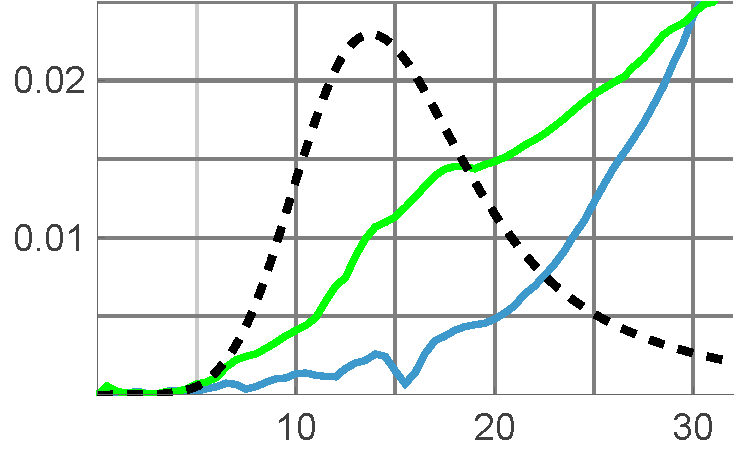
\includegraphics[width=0.458\linewidth]{figures/7-1.pdf}}
		\put(70,55){$5\Omega$}
		\put(95,45){$4\Omega$}
		\put(20,50){$(7,\,1)$}
		\put(18,25){\textbf{e)}}

		\put(130,0){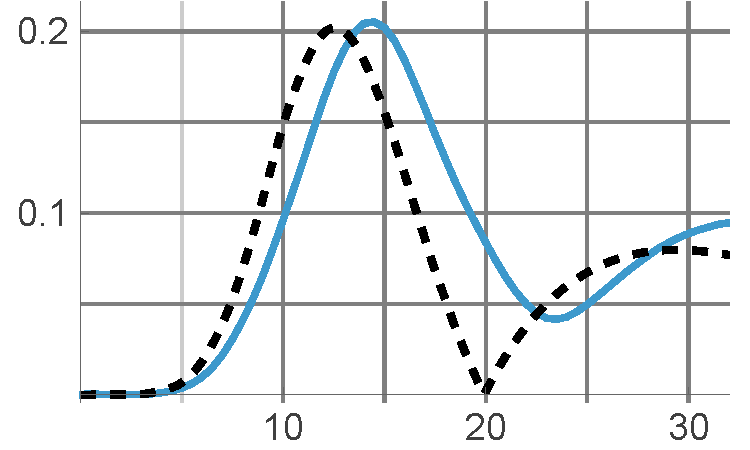
\includegraphics[width=0.46\linewidth]{figures/7-2.pdf}}
		\put(197,50){$6\Omega, \ \ (7,\,2)$}
		\put(145,35){\textbf{f)}}

	\end{picture}

	% TODO: [Amplitude comparison] Give radial/velocity units and state whether each
	% theoretical profile is independently rescaled to the data. An unforced
	% eigenproblem predicts shapes and frequencies, not absolute amplitudes; specify
	% which normalization is retained when comparing measured amplitudes across panels.
	\caption{Comparison of theoretical radial profiles of the magnitude of $u_\varphi$ (dashed lines) with experimentally measured amplitudes of $u_\varphi$ oscillations at a fixed frequency and azimuthal mode number $m$ (solid lines). Labels $l\Omega$, with positive integer $l$, indicate the measured frequencies; see the spectrum in Figure~\ref{fig:spectrum}. Theoretical modes are labeled by $(m,\,n)$, as in Figure~\ref{fig:wave-theory}.}
	\label{fig:modes-exp}
\end{figure}



\section{Comparison of experiment and theory}
\label{sec:results}

% TODO: [Geometry/mode identification] In a square basin m labels an azimuthal
% Fourier component, not generally an eigenmode. Discuss mixing allowed by the
% fourfold symmetry (including m values differing by 4), and justify one-to-one
% assignments to cylindrical eigenmodes, especially for modes that reach the walls.
We now compare the experimental observations with the theoretical predictions. Because the theory assumes a circular basin whereas the experimental basin is square, only qualitative agreement between the modes is expected.

% TODO: [Profile evidence] Quantify profile/node-position uncertainties and the
% criterion for assigning n when the outer part r>32 cm is unobserved. State how
% a single free-mode profile is distinguished from a forced superposition, and
% which evidence supports wall-reaching behavior outside the measured radial range.
The experimentally measured modes are forced oscillations, so their frequencies are integer multiples $l\Omega$ of the angular velocity $\Omega$ of the disk; see the spectrum in Figure~\ref{fig:spectrum}. Figure~\ref{fig:modes-exp} shows the radial profiles $|u_\varphi|$ for selected modes. Measurements along the radial coordinate $r$ were restricted to radii for which a full circle of radius $r$ fits within the basin, that is, $r<35\,\text{cm}$. We plot the wave fields only up to a radius of $32\,\text{cm}$ because a turbulent boundary layer of thickness $\approx 3\,\text{cm}$ near the sidewalls introduces unacceptably large measurement errors. For the mode $(m,n) = (3,3)$, for example, Figure~\ref{fig:modes-exp}(a) shows good quantitative agreement. The first node of the theoretically calculated profile lies slightly closer to the basin center than the corresponding node of the measured profile. The same pattern holds for other modes with low radial mode numbers $n=2,3$ at different $m$; see, for example, Figure~\ref{fig:modes-exp}(f). We use this pattern to assign the radial mode numbers $n$ to modes with higher $n$, as shown in Figures~\ref{fig:modes-exp}(b) and \ref{fig:modes-exp}(d), although the agreement in these cases is qualitative rather than quantitative.

% TODO: [Resonant response] Amplitude depends on forcing strength, modal overlap,
% normalization, and damping as well as detuning. Demonstrate that these factors
% are controlled or estimated before using amplitudes of different modes/harmonics
% as evidence for their relative proximity to resonance.
The closer the forcing frequency $l\Omega$ is to a mode's eigenfrequency, the larger its amplitude. The relative amplitudes of the measured modes shown in Figure~\ref{fig:modes-exp} therefore indicate their proximity to resonance. In Figure~\ref{fig:map}, filled circles represent all wave fields measured at fixed $m$ and $l$, with color indicating intensity. Curved lines connect the theoretically calculated modes to the corresponding experimentally observed wave fields.

% TODO: [Trapped-mode search/detuning] In map.tex's Hz convention, (7,1) is at
% 1.749139 Hz and the nearest harmonic is 6*Omega=1.857343 Hz, not either of the
% 4*Omega and 5*Omega fields shown in panel (e). The (7,2) mode at 1.881346 Hz is
% much closer to 6*Omega. Compare detunings with independently estimated damping
% widths and test whether a weak (7,1) contribution is hidden in panel (f).
% TODO: [Non-detection] Give the tested frequency range, sensitivity and modal
% separation procedure for m=7 and m=8. Non-detection does not establish zero
% excitation or uniquely identify a sidewall-mediated forcing mechanism; exclude
% detuning, weak overlap, damping, and model/geometry shifts as alternatives.
After establishing the correspondence between modes, we sought to observe modes radially localized by the mean flow. According to Figure~\ref{fig:map}, the lowest azimuthal mode number of interest is $m=7$. However, the localized mode was not detected; see Figure~\ref{fig:modes-exp}(e). Instead, we observed strongly delocalized surface oscillations with relatively low amplitudes. This cannot be explained by the relatively large value of $m$, since the mode $(7,2)$ is clearly observed in Figure~\ref{fig:modes-exp}(f). The same is true for $m=8$; the radial profile of the theoretically calculated mode $(8,1)$ is plotted in Figure~\ref{fig:wave-theory}. We conclude that localized modes are not excited in our experiment. Because the distinguishing feature of localized modes is their lack of interaction with the sidewalls, we infer that the excitation mechanism relies on fluid interaction with the sidewalls.

% TODO: [Mode cutoff] Derive or identify the empirical basis for sqrt(m^2+n^2)
% as a wavelength proxy: azimuthal scale involves m/r, whereas radial scale
% depends on turning points and nodal spacing. Evaluate the local capillary ratio
% and measurement resolution for these modes, and distinguish excluded modes from
% the higher-index theoretical modes still illustrated in the map/profile figures.
When $\sqrt{m^2+n^2}\gtrsim 9$, the nodes in the measured profiles are typically less pronounced, making comparison with the theoretical predictions ambiguous. This may reflect the limited accuracy of our measurements or the simultaneous excitation of multiple eigenmodes. These mode numbers correspond to relatively short waves for which capillary effects are appreciable, so we do not consider these modes further.


\section{Conclusion}
\label{sec:conclusion}

% TODO: [Scope of conclusion] The homogeneous eigenvalue calculation establishes
% mode existence, not that both families should be excited by the actual forcing.
% Separate this prediction from the proposed excitation mechanism and the limits
% of non-detection. Localized modes have evanescent tails, not identically zero
% sidewall interaction; quantify negligible coupling rather than assuming its absence.
We experimentally observe surface waves propagating against a ring current established in a closed square basin. The slight tilt of the disk that generates the ring current also provides the wave forcing. A systematic comparison with numerical results obtained from our theory supports the experimental observations. The theory predicts that both delocalized and trapped modes should be excited in the experiment. However, only delocalized modes are detected. We propose that trapped modes are not excited by the chosen forcing mechanism because they do not interact with the basin sidewalls. Future experiments should investigate which modes are excited in a cylindrical basin and how trapped modes can be excited.



\section{Acknowledgments}

Ivan A. Vointsev was supported by the Basic Research Program of HSE University (project HSE-BR-2025-57).



\bibliography{wave-trapping}

\end{document}

% Physics/mathematics review: the added TODO comments are nonprinting author queries.
